\chapter{Stratified spaces}
\label{lecture:18}
\remyquote{Now it's just three weeks of me having fun.}

\section{Stratified spaces and exodormy}
In \cref{lecture:4}, we discussed the following diagram:
\begin{equation*}
    \begin{tikzcd}
        \catSheaf(X) \ar[r, "\simeq"] & \catLocalHomeomorphism_{/X} \\
        \catLocallyConstantSheaf(X) \ar[u, inclusion] \ar[r, "\simeq"'] & \catCoveringSpace_{/X} \ar[u, inclusion] \ar[r, "\simeq"'] & \catFunctor(\deloop\homotopy[1](X,x_0),\catSet)
    \end{tikzcd}
\end{equation*}
(To avoid choosing a basepoint, we can replace \(\deloop\homotopy[1](X,x_0)\) by the fundamental groupoid\footnote{If you want to be fancy, this is the homotopy \(1\)-category of the fundamental \(\infty\)-groupoid of \(X\) (modelled as a Kan complex by the singular simplicial set of \(X\)).} \(\Pi_1(X)\), whose objects are the points \(x\in X\) and whose maps \(x\to y\) are homotopy classes of paths from \(x\) to \(y\).)

We will discuss in the following weeks in more detail the question: is there something in the top right spot?
This will be partially answered by \emph{exodromy}, but only for \emph{constructible sheaves}.
In this week's lecture, we discuss the topological setup, and next week we introduce constructible sheaves and discuss exodromy.

\section{Stratifications}
The most basic version of a stratification (a notion we will introduce momentarily) is a \emph{filtration}.

\begin{defn}
A \emph{filtration} of a topological space \(X\) is a sequence of closed subspaces
\[ \emptyset=Z_{-1}\subseteq Z_0\subseteq Z_1\subseteq\ldots\subseteq X \]
indexed by the natural numbers (and \(-1\), but we always set \(Z_{-1}\coloneq\emptyset\)) such that \(X=\bigcup_{i\in\bb N}Z_i\).
\end{defn}

\begin{exmp}
One may filter the \(n\)-cube \([0,1]^n\) by
\[ Z_i \coloneq \setpred{(x_1,\ldots,x_n)}{\#\{x_j\neq 0,1\}\leq i}\text{.} \]
The picture for \(n=2\) is as follows:
\begin{center}
  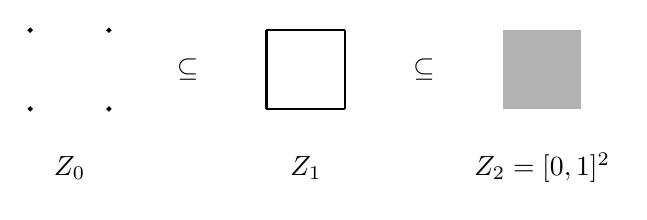
\begin{tikzpicture}
    \draw[fill] (0, 0) circle (0.025);
    \draw[fill] (0, 1) circle (0.025);
    \draw[fill] (1, 0) circle (0.025);
    \draw[fill] (1, 1) circle (0.025);
    \node at (0.5, -.75) {\(Z_0\)};
    \node at (2, 0.5) {\(\subseteq\)};
    \draw[thick] (3, 0) -- (3, 1);
    \draw[thick] (3, 0) -- (4, 0);
    \draw[thick] (3, 1) -- (4, 1);
    \draw[thick] (4, 0) -- (4, 1);
    \node at (3.5, -.75) {\(Z_1\)};
    \node at (5, 0.5) {\(\subseteq\)};
    \fill[black!30] (6, 0) rectangle (7, 1);
    \node at (6.5, -.75) {\(Z_2=[0,1]^2\)};
  \end{tikzpicture}
\end{center}
\end{exmp}

\begin{exmp}
Generalising the previous example, a CW-complex \(X\) is filtered by its skeleta:
\[ X_0 \subseteq X_1 \subseteq X_2 \subseteq\ldots \subseteq X\]
The \(i\)-skeleton \(X_i\) is the union of the cells of dimension \(\leq i\).
\end{exmp}

It is often convenient to describe the locally closed subsets \(Z_i\setminus Z_{i-1}\) instead of the subsets \(Z_i\).
This is captured in the following definition.

\begin{defn}\label{defn:N-stratification}
An \emph{\(\bb N\)-stratification} of a topological space \(X\) is a decomposition
\[ X = \coprod_{i\in\bb N}X_i \]
into locally closed subsets \(X_i\) such that \(\overline{X_i}\subseteq X_{\leq i}\coloneq\bigcup_{j\leq i}X_j\).
The disjoint union here is a disjoint union of \emph{sets}; \(X\) need not have the disjoint union topology with respect to the \(X_i\).
\end{defn}

\begin{lem}
Let \(X=\coprod_{i\in\bb N}X_i\) be a decomposition of a topological space into subsets \(X_i\).
Then the following are equivalent:
\begin{enumerate}
\item the subsets \(X_i\) are locally closed and \(\overline{X_i}\subseteq X_{\leq i}\) (the decomposition is an \(\bb N\)-stratification in the above sense);
\item the subsets \(X_{\leq i}\) are closed.
\end{enumerate}
\end{lem}
\begin{proof}
If the latter holds, then the \(X_i=X_{\leq i}\setminus X_{\leq i-1}\) are locally closed and since \(X_i\) is contained in the closed subset \(X_{\leq i}\), so is its closure.
Conversely, if the former statement holds, then
\[ \overline{X_{\leq i}} = \bigcup_{j\leq i}\overline{X_j} \subseteq \bigcup_{j\leq i}X_{\leq j} = X_{\leq i}\text{,} \]
so the \(X_{\leq i}\) are closed.
\end{proof}

\begin{lem}
Filtrations of a topological space \(X\) correspond bijectively to \(\bb N\)-stratifications of \(X\) via the maps
\begin{align*}
  (Z_0\subseteq Z_1\subseteq\ldots) & \mapsto \bigl(X=\coprod_{i\in\bb N}Z_i\setminus Z_{i-1}\bigr)\text{,} \\
  (X_{\leq 0}\subseteq X_{\leq 1}\subseteq\ldots) & \mapsfrom \bigl(X=\coprod_{i\in\bb N}X_i\bigr)\text{.}
\end{align*}
\end{lem}
\begin{proof}
If \((Z_0\subseteq Z_1\subseteq\ldots)\) is a filtration of \(X\), then \(Z_i\setminus Z_{i-1}\) is locally closed, and \(X_{\leq i}=\bigcup_{j\leq i}Z_j\setminus Z_{j-1}=Z_i\) is closed.
Conversely, if \(X=\coprod_{i\in\bb N}X_i\) is an \(\bb N\)-stratification, then the \(X_{\leq i}\) are closed, and \(\bigcup_{i\in\bb N}X_{\leq i}=X\).
Clearly, \(X_{\leq i}\setminus X_{\leq i-1}=X_i\).
We have thus seen that the maps are well-defined and are inverses.
\end{proof}

It is often useful to allow other posets than \(\bb N\).

\begin{defn}
The \emph{Alexandroff topology} on a poset \(P\) is the topology whose opens are the \emph{upwards closed subsets} (also called \emph{cosieves}): those subsets \(U\subseteq P\) such that if \(p\in U\) and \(p\leq q\in P\), then \(q\in U\).
\end{defn}

\begin{rmk}
The Alexandroff topology is a topology; in fact, both arbitrary unions and arbitrary intersections of cosieves are cosieves.
The closed subsets are the \emph{downward closed subsets} (\emph{sieves}), which also form a topology: the Alexandroff topology on \(P\opp\).
\end{rmk}

\begin{exmp}
For \(P=[1]=\{0<1\}\), the opens in the Alexandroff topology on \(P\) are \(\emptyset\), \(\{1\}\) and \(\{0,1\}\), so this is the Sierpiński space.
\end{exmp}

\begin{exmp}
The sets \(P_{\geq p}=\setpred{q\in P}{q\geq p}\) are open, and \(P_{\leq p}\) is closed.
Likewise, \(P_{>p}\) is open and \(P_{<p}\) is closed.
The singletons \(\{p\}=P_{\geq p}\cap P_{\leq p}\) are locally closed.
\end{exmp}

\begin{defn}
Let \(X\) be a topological space and \(P\) a poset.
Then a \emph{\(P\)-stratification} on \(X\) is a continuous map \(f\colon X\to P\) (where \(P\) is endowed with the Alexandroff topology).
A \emph{stratification} on \(X\) is a \(P\)-stratification for some \(P\).
\end{defn}

\begin{exmp}
If \(P=\bb N\), then a continuous map \(f\colon X\to\bb N\) is a the same thing as an \(\bb N\)-stratification in the sense of \cref{defn:N-stratification}: the closed subsets (sieves) on \(\bb N\) are exactly \(\bb N_{\leq i}\) for some \(i\in\bb N\), and \(\emptyset\) and \(\bb N\).
\end{exmp}

\begin{exmp}
If \(P=[1]\), we saw on Homework~1 that a \(P\)-stratification \(f\colon X\to P\) is given by an open subsets \(U\coloneq f\inv(1)\) (with closed complement \(Z\coloneq f\inv(0)\))
\end{exmp}

\begin{defn}
Given a map \(f\colon X\to P\) (not necessarly continuous) from a topological space \(X\) to a poset \(P\), we write
\[ X_{\geq p} \coloneq f\inv(P_{\geq p})\text{,} \quad X_{>p}\coloneq f\inv(P_{>p})\text{,} \quad X_{\leq p}\coloneq f\inv(P_{\leq p})\text{,} \quad X_{<p}\coloneq f\inv(P_{<p})\text{.} \]
The set \(X_p\coloneq f\inv(p)\) is called the \emph{\(p\)th stratum}; it is locally closed if \(f\) is continuous.
\end{defn}

\begin{rmk}
Continuity of \(f\colon X\to P\) implies
\[ f(\overline{X_p}) \subseteq \overline{f(X_p)} = \overline{\{p\}} = P_{\leq p}\text{,} \]
so \(\overline{X_p}\subseteq X_{\leq p}\).
The converse holds if \(P=\bb N\) or if \(P\) is finite, but not in general (see Additional exercise~18.4).
\end{rmk}

\todo{example \(n\)-cube}

\begin{exmp}
The unit interval \(I=[0,1]\) can be stratified over \([1]\) as in the following picture:
\begin{center}
  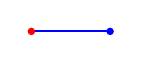
\begin{tikzpicture}
    \draw[thick,blue] (0,0)--(1,0);
    \draw[fill,red] (0,0) circle (0.04);
    \draw[fill,blue] (1,0) circle (0.04);
  \end{tikzpicture}
\end{center}
sending the left endpoint \(0\) (red) to \(0\) and the rest of the interval to \(1\).
\end{exmp}

\begin{exmp}
The circle can be stratified as in the picture
\begin{center}
  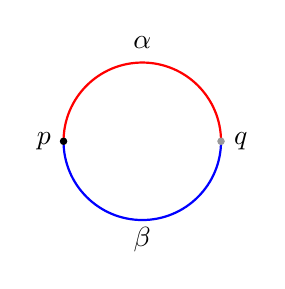
\begin{tikzpicture}
    \draw[thick,red] (-1,0) arc[start angle=180, end angle=0, x radius=1, y radius=1];
    \draw[thick,blue] (-1,0) arc[start angle=180, end angle=360, x radius=1, y radius=1];
    \draw[fill] (-1,0) circle (0.04);
    \draw[fill,black!40] (1,0) circle (0.04);
    \node at (-1.25,0) {\(p\)};
    \node at (1.25,0) {\(q\)};
    \node at (0,1.25) {\(\alpha\)};
    \node at (0,-1.25) {\(\beta\)};
  \end{tikzpicture}
\end{center}
over the poset with elements \(\{p,q,\alpha,\beta\}\) with \(p<\alpha\), \(p<\beta\), \(q<\alpha\) and \(q<\beta\).
\end{exmp}

\begin{exmp}
We can stratify the \(2\)-sphere over \([2]=\{0<1<2\}\) as in the following picture:
\begin{center}
  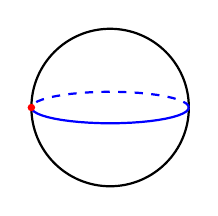
\begin{tikzpicture}
    % inspiration from https://people.uncw.edu/hermanr/phy495/Bloch_Sphere.pdf
    \draw[thick] (0,0) circle (1);
    \draw[thick,blue] plot[domain=pi:2*pi] ({cos(\x r)},{.2*sin(\x r)});
    \draw[thick,dashed,blue] plot[domain=0:pi] ({cos(\x r)},{.2*sin(\x r)});
    \draw[fill,red] (-1, 0) circle (0.04);
  \end{tikzpicture}
\end{center}
sending the red point to \(0\), the blue equator to \(1\), and the two hemispheres to \(2\).
We can also stratify the \(2\)-sphere over the poset with elements \(\{0,1,2,2'\}\) with \(0<1\), \(1<2\) and \(1<2'\) by sending the upper hemisphere to \(2\) and the lower hemisphere to \(2'\).
\end{exmp}

\begin{exmp}
The plane \(\bb R^2\) can be stratified as in the picture
\begin{center}
  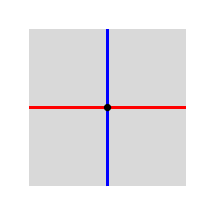
\begin{tikzpicture}
    \fill[black!15] (-1,-1) rectangle (1,1);
    \draw[thick,blue] (0,-1) -- (0,1);
    \draw[thick,red] (-1,0) -- (1,0);
    \draw[fill] (0,0) circle (0.04);
  \end{tikzpicture}
\end{center}
over the poset with elements \(\{0,1,1',2\}\) with \(0<1\), \(0<1'\), \(1<2\) and \(1'<2\) by sending the origin to \(0\), the \(x\)-axis minus the origin to \(1\), the \(y\)-axis minus the origin to \(1'\) and the rest to \(2\).
\end{exmp}

\begin{rmk}
The examples above all satisfy extra properties:
\begin{enumerate}
\item if \(p\leq q\), then \(X_p\cap\overline{X_q}\neq\emptyset\);
\item \(\overline{X_p}\) is a union of strata (\(X_p\cap\overline{X_q}\neq\emptyset\) implies \(X_p\subseteq\overline{X_q}\)).
\end{enumerate}
Together, these properties are equivalent to \(\overline{X_q}=X_{\leq q}\); this condition is called the `axiom of the frontier'.
We will not explicitly impose this condition, but many authors \emph{do} assume the axiom of the frontier or other additional aximos.
\end{rmk}

\todo{write}

\section{Conical stratifications}
\begin{defn}
The \emph{left cone} \(\leftcone{\cat C}\) on a category \(\cat C\) is the category with objects \(\cat C\cotimes\{-\infty\}\) and maps
\[ \Hom[\leftcone{\cat C}](x,y) =
  \begin{cases}
    \Hom[\cat C](x,y) & \text{if } x,y\in\cat C\text{,} \\
    \terminal & \text{if } x = -\infty\text{,} \\
    \emptyset & \text{if } x\in\cat C, y = -\infty\text{.}
  \end{cases}
\]
Dually, the \emph{right cone} \(\rightcone{\cat C}\) of \(\cat C\) is the category \((\leftcone{(\cat C\opp)})\opp\).
\end{defn}

The left cone of a category \(\cat C\) is obtained by formally adjoining an initial object to \(\cat C\); dually, the right cone of \(\cat C\) is \(\cat C\) where a terminal object is formally adjoined.

\begin{rmk}
If \(\cat C\) is a preorder, that is, if \(\#\Hom[\cat C](x,y)\leq 1\) for all \(x,y\in\cat C\), then so is the left cone \(\leftcone{\cat C}\).
If \(\cat C\) is a poset (that is, a preorder such that \(\Hom[\cat C](x,y)\times\Hom[\cat C](y,x)\neq\emptyset\) implies \(x=y\)), then so is the left cone \(\leftcone{\cat C}\).
\end{rmk}

We will only deal with left cones of posets in this and next week's lecture, but since the definition makes sense for all categories, we have presented it in this generality.

\begin{exmp}
For the totally ordered set \([n]=\{0<1<\ldots<n\}\) with \(n+1\) elements, we have  
\[ \leftcone{[n]} \cong [n+1] \cong \rightcone{[n]}\text{.} \]
\end{exmp}

\begin{defn}
The \emph{cone} \(CX\) of a topological space \(X\) is the space \(CX\coloneq (X\times\bb R_{>0})\cup\{*\}\) where \(U\subseteq CX\) is open if and only if \(U\cap(X\times\bb R_{>0})\) is open and if \(*\in U\) implies that \(X\times(0,\epsilon)\subseteq U\) for some \(\epsilon>0\).
\end{defn}

\begin{rmk}
Usually, one defines the cones as the pushout \(X\times\bb R_{\geq 0}\pushout{X\times\{0\}}\{*\}\).
Then the second condition becomes: if \(*\in U\), then for all \(x\in X\) there exists an open neighbourhood \(V_x\subseteq X\) of \(x\) and an \(\epsilon_x>0\) such that \(V_x\times(0,\epsilon_x)\subseteq U\).

The natural map \((X\times\bb R_{\geq 0})\pushout{X\times\{0\}}\{*\}\to CX\) is a homeomorphism if \(X\) is compact, but not when \(X=\bb R\) for instance.
\end{rmk}

\begin{defn}
If \(f\colon X\to P\) is a stratification, define the \emph{left cone} \(\leftcone{f}\colon CX\to\leftcone{P}\) of \(f\) by \(*\mapsto-\infty\) and \((x,t)\mapsto f(x)\) for \((x,t)\in X\times\bb R_{>0}\).
\end{defn}

This definition makes sense as the point \(*\) is closed, and contained in the closure of \(Z\times\bb R_{>0}\) for any closed subset \(Z\subseteq X\).

The picture for the left cone of a \(P\)-stratification of the circle is as follows:
\begin{center}
  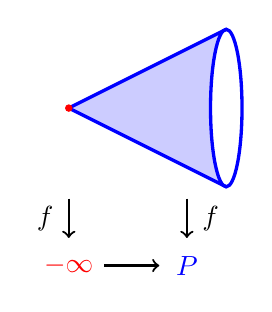
\begin{tikzpicture}
    \draw[fill,blue!20] (0,0) -- (2,1) -- (2,-1);
    \draw[blue, very thick, fill=white] (2,0) ellipse [x radius=.2, y radius=1];
    \draw[blue, very thick] (0,0) -- (2,1);
    \draw[blue, very thick] (0,0) -- (2,-1);
    \draw[red, fill] (0,0) circle (0.04);
    \draw[thick,->] (0,-1.15) -- (0,-1.65);
    \node at (-.3,-1.40) {\(\leftcone{f}\)};
    \node[red] at (0,-2) {\(-\infty\)};
    \draw[thick,->] (1.5,-1.15) -- (1.5,-1.65);
    \node at (1.8,-1.40) {\(f\)};
    \node[blue] at (1.5,-2) {\(P\)};
    \draw[thick,->] (.45,-2) -- (1.15,-2);
  \end{tikzpicture}
\end{center}

\begin{defn}
A stratification \(f\colon X\to P\) is \emph{conical} if every point \(x\in X\) has an open neighbourhood \(U\subseteq X_{\leq p}\) where \(p\coloneq f(x)\) such that \(f|_U\colon U\to P_{\geq p}\) is isomorphic to \(Z\times CY\) for some \(P_{>p}\)-stratified space \(Y\) and a path connected and locally path connected \footnote{This should probably include `semi-locally simply connected'.} space \(Z\).
Such a neighbourhood \(U\) is called a \emph{basic neighbourhood}.
\end{defn}

Note for this definition that \(\leftcone{(P_{>p})}\cong P_{\geq p}\).

We state the following fact without explaining what we mean precisely.
\begin{prop}
Stratifications by closed embedded submanifolds are conical.
\end{prop}

\todo{Examples and counterexamples}

\todo{write}

%%% Local Variables:
%%% mode: latex
%%% TeX-master: "../main"
%%% End:
